\documentclass[crop,tikz]{standalone}
\usepackage{tikz}
% \usepackage{pgfmath} % For random numbers
\usetikzlibrary{calc}
\usepackage{pgf}
\begin{document}


% \usepackage{tikz}
% \usepackage{pgfmath}

% \begin{document}

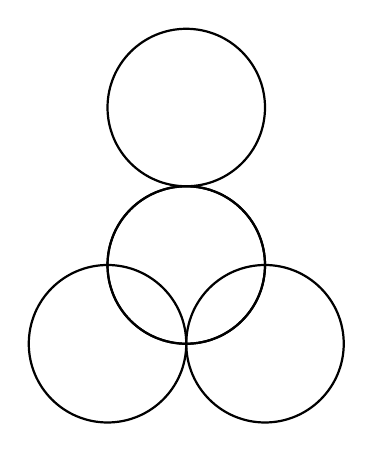
\begin{tikzpicture}
    \pgfmathsetseed{1234} % Set seed for reproducibility

    % Parameters
    \def\ncircles{10} % Number of circles
    \coordinate (currentcenter) at (0, 0); % Initial circle center
    \pgfmathsetmacro{\currentradius}{1}; % Initial circle radius

    % Draw the first circle
    \draw[thick] (currentcenter) circle (\currentradius);

    % Keep track of the circle information
    \pgfmathsetmacro{\xpos}{0}; % x-coordinate
    \pgfmathsetmacro{\ypos}{0}; % y-coordinate

    % Loop to draw the remaining circles
    \foreach \i in {1,...,\ncircles} {
%         % Randomly choose a new radius between 0.5 and 1.5
        % \pgfmathrandombetween{0.5}{1.5};
        % \pgfmathsetmacro{\newradius}{\pgfmathresult / 10};

        \pgfmathsetmacro{\newradius}{random(0.5,1.5))}
        % \node[draw] {\newradius};
% % 
%         % Randomly decide the new circle's direction: left, right, up, or do
        % \pgfmathsetmacro{\direction}{1}
        \pgfmathrandominteger{\direction}{1}{4}
        % \node[draw] {\direction};

        \ifnum\direction=1
            % Right
            \pgfmathsetmacro{\newx}{\xpos + \currentradius + \newradius}
            \pgfmathsetmacro{\newy}{\ypos}
        \else\ifnum\direction=2
            % Left
            \pgfmathsetmacro{\newx}{\xpos - \currentradius - \newradius}
            \pgfmathsetmacro{\newy}{\ypos}
        \else\ifnum\direction=3
            % Up
            \pgfmathsetmacro{\newx}{\xpos}
            \pgfmathsetmacro{\newy}{\ypos + \currentradius + \newradius}
        \else
            % Down
            \pgfmathsetmacro{\newx}{\xpos}
            \pgfmathsetmacro{\newy}{\ypos - \currentradius + \newradius}
        \fi\fi\fi

%         % Update coordinates and radius
        \coordinate (currentcenter) at (\newx, \newy);
        \draw[thick] (currentcenter) circle (\newradius);

        \xdef\xpos{\newx}
        \xdef\ypos{\newy}
        \xdef\currentradius{\newradius}
    }
\end{tikzpicture}

\end{document}

\end{document}